
\chapter{Methods}
\label{cha:method}

\section{Overall pipeline architecture}

By joining all the parts exposed in the previous chapters, the resulting pipeline proposed as a solution is shown in Figure \ref{fig:sol_pipeline}. Based on the flow presented, the obtained results are summarised in the following sections.

\begin{figure}[H]
	\centering
	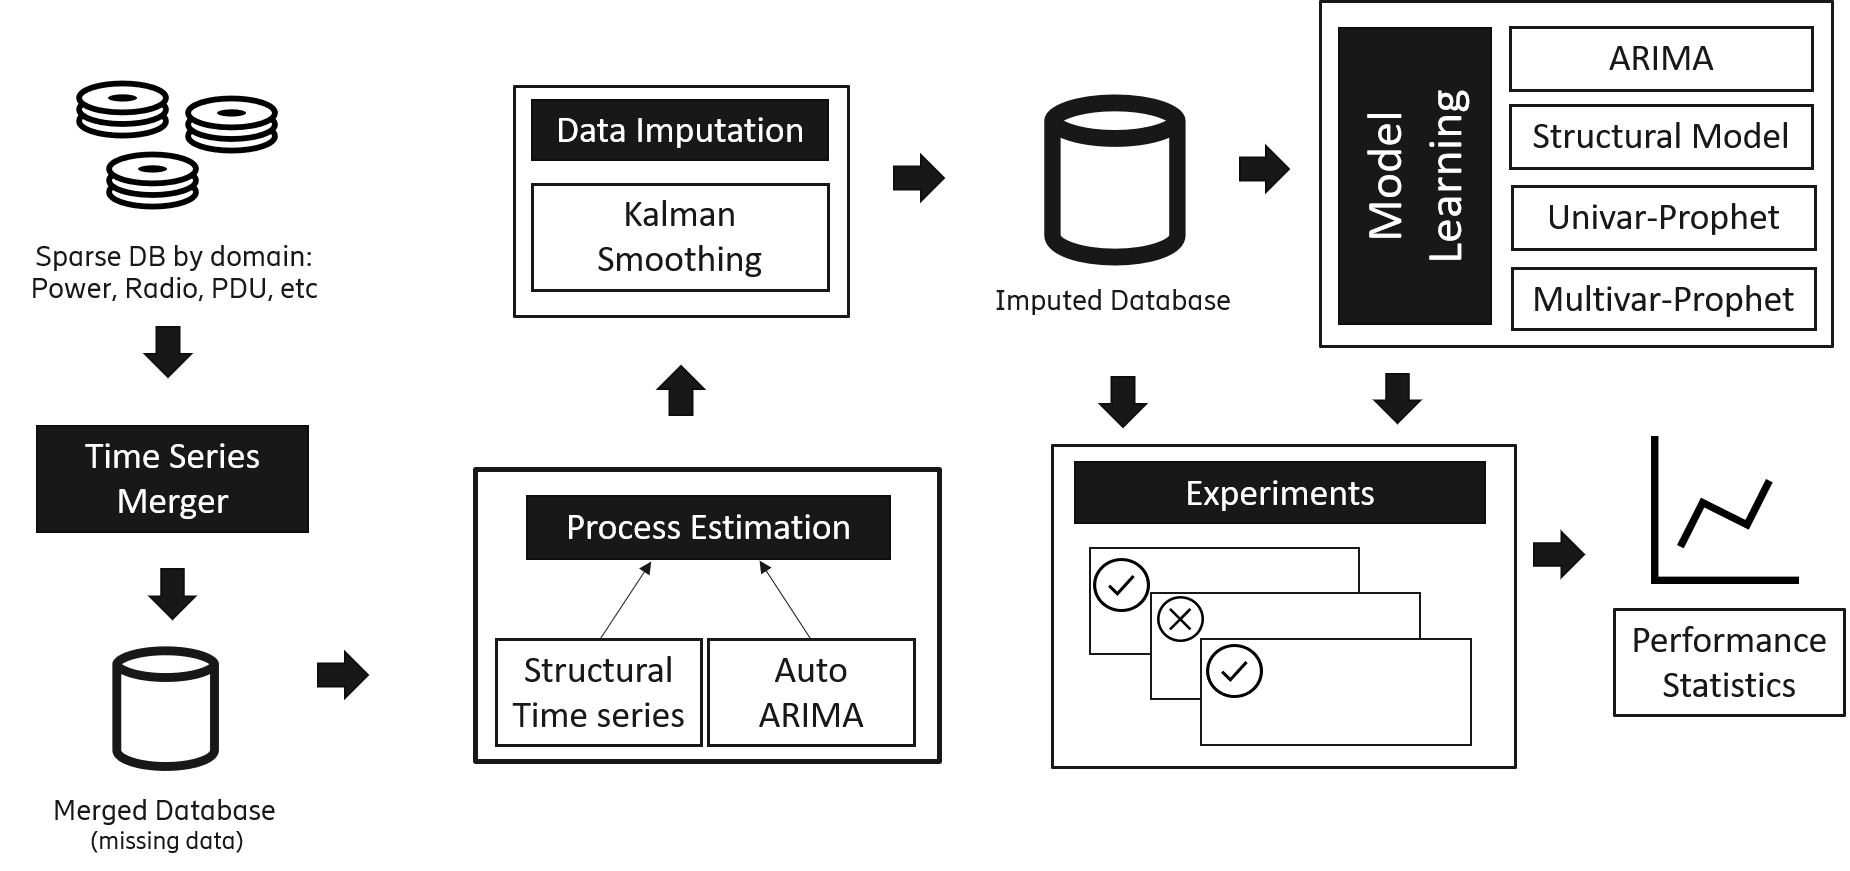
\includegraphics[width=1\linewidth]{pipeline_v4}
	\caption{Overall pipeline architecture}
	\label{fig:sol_pipeline}
\end{figure}


\section{Database building and time series merging}
\label{sec:db_building}

As mentioned, the data is sparse across several files depending on its domain. Therefore, all the data has been merged into one consolidated database to make it more manageable to handle. Then, there is the problem of determining the best approach to join all these data without corrupting its integrity as a valid time series; this means having an invariant sampling time with fully defined observations vectors.

Among the data tables, it can be seen that the two fields that are always present, and therefore are suitable to use as keys to index all the different tables and join them, are the timestamp of the sample and the \ac{rbs} that has produced it. Therefore, the tuples $(\text{date}_i, \text{rbs}_i)$ will be used as keys. This means, having two relations $R(x_1, \ldots, x_n)$ and $S(y_1,\ldots,y_m)$ a third relation could be constructed $Q(z_1, \ldots, z_k) = R \times S$ such that $R(\vec{x}_i) = S(\vec{y}_i$) be the keys \cite{mishra1992join}.

\begin{figure}[H]
	\centering
	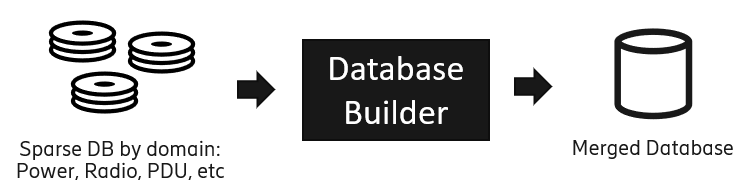
\includegraphics[width=0.55\linewidth]{db_merge_pipeline.png}
	\caption{Database consolidation}
	\label{fig:db_merge}
\end{figure}

In an ideal situation, all the time series for a given \ac{rbs} would have no missing data and identical timestamps, so just intersecting them would result in a complete-time series with equal sampling time, and no information would be lost.  Nonetheless, that is not the current case. As real-world data, technical issues happen now and then. There could be missing samples, or the timestamps between different files are not equidistant and, therefore, a join using them will not perform as expected.

The present work has been implemented mainly in Python with a few exceptions in R. The joining part is not an exception; thus, pandas \texttt{merge} options are available to use: \emph{left, right, outer, inner} or \emph{cross}. Merge operations in pandas work on two sets \cite{reback2020pandas}. Thus, for joining multiple series, successive two-sided \texttt{merge} operations have to be performed.

\subsection{Strategy analysis: Inner join}

An inner join constitutes an intersection between both sets. The implementation in pandas allows indicating the keys to be intersected, and as a result, a tuple is returned containing the matched keys with the remaining members. This can be expressed as the following 

$$Q(date_i, rbs_i,  x_{i_1}, \ldots, x_{i_n}, y_{i_1}, \ldots, y_{i_m}) = $$
$$  R(date_i, rbs_i, x_{i_1}, \ldots, x_{i_n}) \bigcap \
S(date_i, rbs_i, y_{i_1}, \ldots, y_{i_m}) $$

Furthermore, in a more programming-friendly manner, it can also be expressed as a SQL query. The expression above would be as the following and graphically as a 3D Venn diagram as in Figure \ref{fig:inner_join}.

\begin{lstlisting}[language=SQL]
SELECT * 
FROM R 
INNER JOIN S
ON R.date = S.date AND R.rbs = S.rbs;
\end{lstlisting}

The most significant disadvantage of this strategy relies on losing the observations that are not indexed in both datasets. Such nuisance will imply losing the series' head and tails if both series do not have the same start and finish times. If the missing samples are within the series, it will corrupt the constant sampling constraint. Given the amount of data available, these are situations to be avoided.  

\begin{figure}[H]
	\centering
	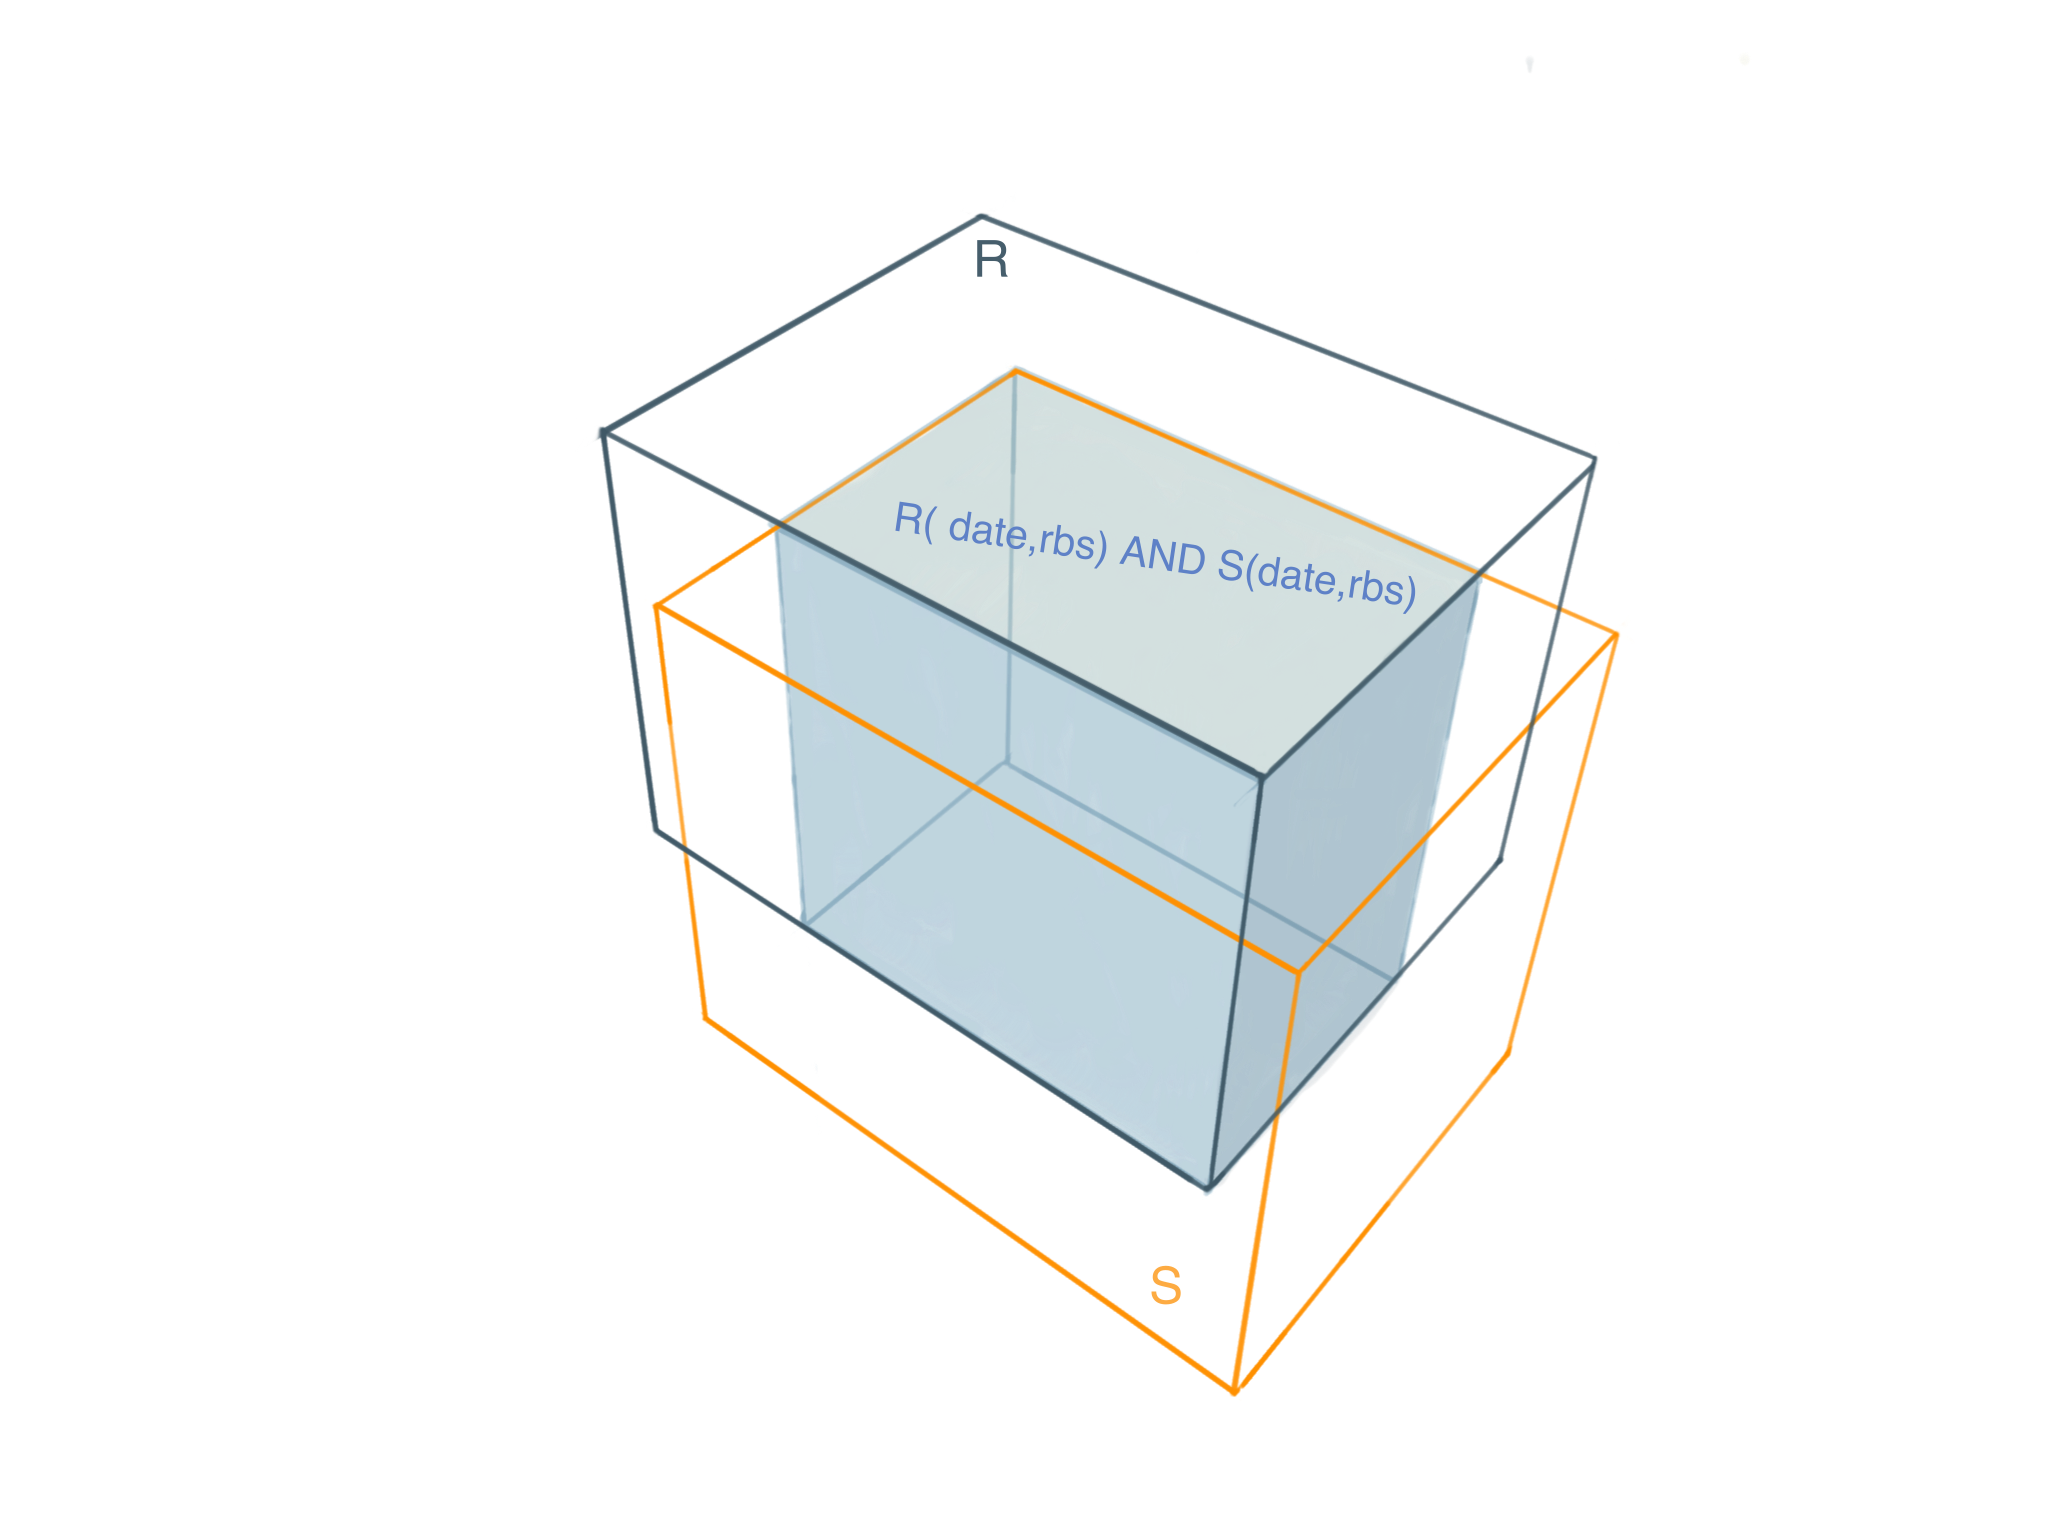
\includegraphics[width=0.90\linewidth]{join_inner}
	\caption{Inner join}
	\label{fig:inner_join}
\end{figure}

 

\subsection{Strategy analysis: Outer join approach}

Whereas an inner join implies an intersection, an outer join can be understood as a union. In pandas, the union implementation is performed in the keys domain, and the rest of the vector is preserved.  If there is some missing value in terms of samples or the full covariates, \texttt{NaN} will be used to fill in.

Given the relations $R$ and $S$ from Section \ref{sec:db_building}:

$$R(date_i, rbs_i, x_{i_1}, \ldots, x_{i_n}), S(date_i, rbs_i, y_{i_1}, \ldots, y_{i_m})$$

The resulting \emph{outer-joined} relation $Q$ on keys $(\text{date}_i, \text{rbs}_i)$

$$Q(date_i, rbs_i) = R(date_i, rbs_i) \bigcup S(date_i, rbs_i)$$

Such that the missing values on each of the relations are declared as NaN

$$Q(x_i) = \text{NaN} , \forall R(y_i) : (date_i, rbs_i) \in S \land (date_i, rbs_i) \notin S$$
$$Q(y_i) = \text{NaN} , \forall S(x_i) : (date_i, rbs_i) \in R \land (date_i, rbs_i) \notin R$$

Again, in a more programming-friendly fashion, the SQL query would look like the following and a more explanatory Venn diagram as in  \ref{fig:outer_join}.

\begin{lstlisting}[language=SQL]
SELECT *
FROM R
FULL OUTER JOIN S
ON R.date = S.date AND R.rbs = S.rbs;
\end{lstlisting}


\begin{figure}[H]
	\centering
	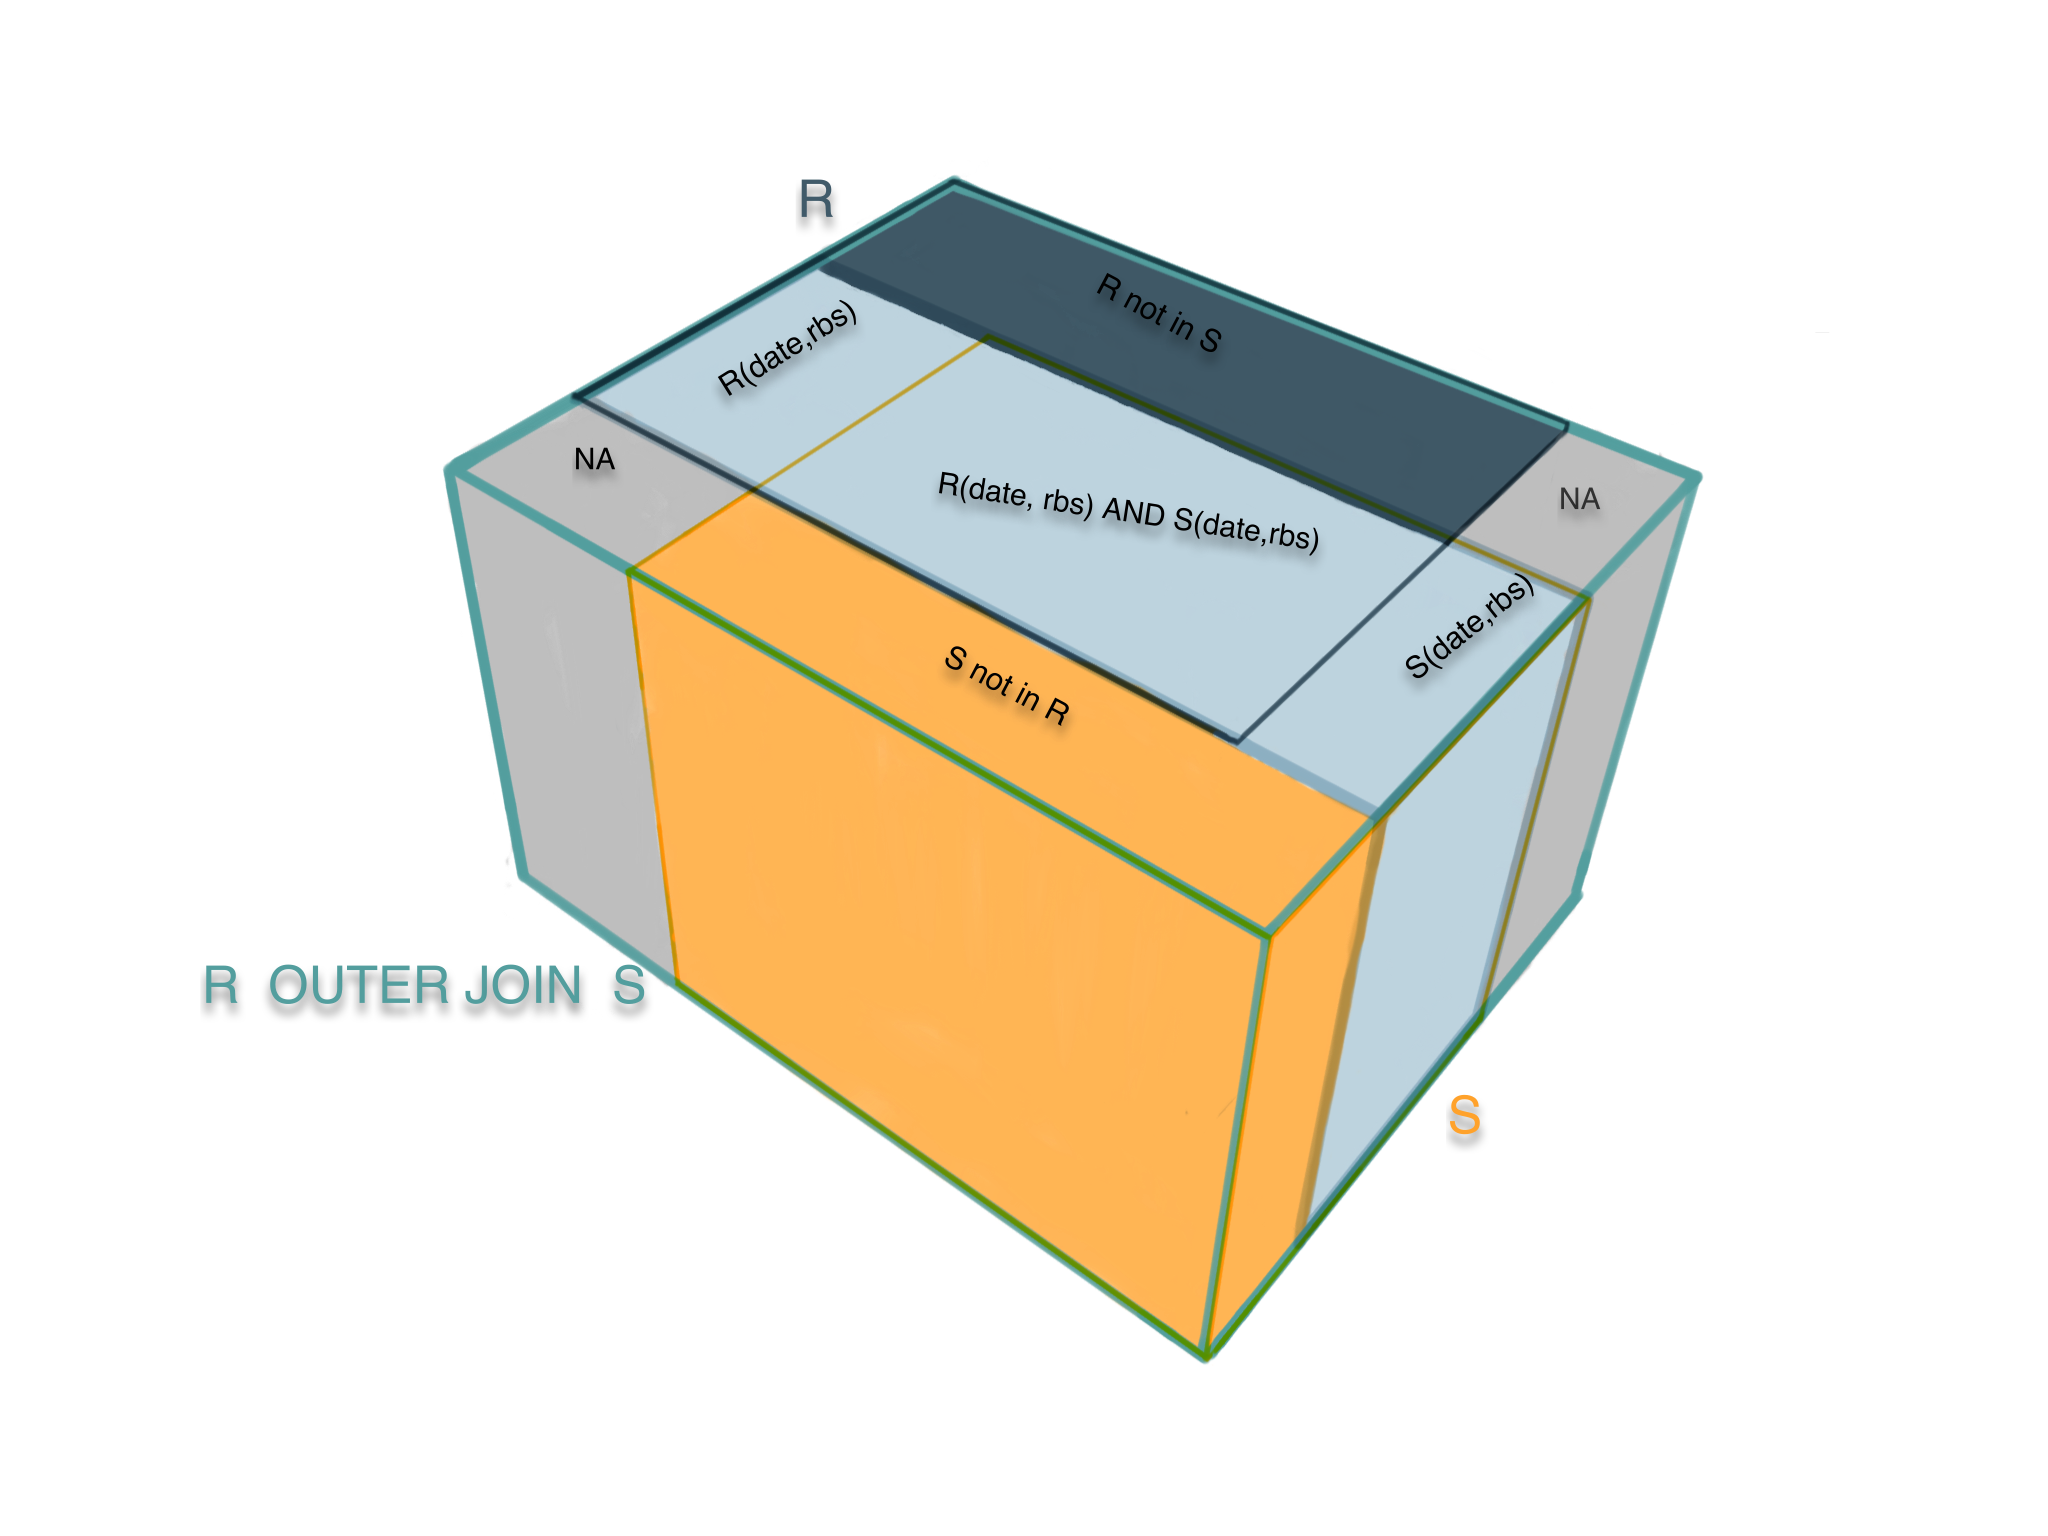
\includegraphics[width=0.90\linewidth]{join_outer}
	\caption{Outer join}
	\label{fig:outer_join}
\end{figure}

The drawback of this approach is related to its insertion of NaNs, which will imply either postprocessing after merging all the time series or preprocessing before the learning stage.

\subsection{Chosen strategy}

Given the analysis, it has been decided that not losing information is more critical than having to dedicate efforts to postprocessing it later to handle the non-computable values. Therefore, the outer join approach will be used for the following steps.

\section{Data Imputation}

As in the previous step, and based on time constraints, it has been decided not to implement algorithms from scratch but rely on existing known packages to avoid investing in developing time. 

Moritz et al. have analysed several univariate time series imputation implementations in R \cite{MoritzComparison}, which results later have been compiled in the \texttt{imputeTS} R package \cite{imputeTS}. Therefore, it is reasonable to rely on their work and use their results to decide which imputing strategy should be taken. 
Thus, for the current work, the \texttt{imputeTS} package will estimate a structural time series model from the data and then perform the Kalman smoothing to fill the gaps. 

It should be noted that before performing the Kalman smoothing, a state representation of the model is needed, \texttt{imputeTS} supports Auto-ARIMA state-space estimation and structural time series model fitted by maximum likelihood. In addition, it should be mentioned that the development has been mainly done in Python. Nonetheless, for this phase, an R package will be called from Python using the \texttt{rpy2} module as an interface to bounce between both languages.

\subsection{Auto-ARIMA algorithm}

Despite the fact that in the library the procedure is called \emph{auto-ARIMA}, it does also support SARIMA models.

The main goal of auto-tuning these models is to choose the appropriate $p, q, d, P, Q$ and $D$ values so the model can make a good approximation of the process. If $d$ and $D$ are known, $p, q, P, Q$ can be selected by using an information criterion such as the \ac{aic} \cite{Akaike1998}:

\begin{equation}
	\text{AIC} = -2\log(L) + 2(p+q+P+Q+k)
\end{equation}

Where $k=1$ if $c\neq0$ in equation (\ref{eq:sarima}) and $0$ otherwise, and $L$ is the maximised likelihood of the model fitted to $(1-B)^d (1-B^s)^D \{Y_t\}$ \cite{autoarimaLib}.  

\texttt{ImputeTS} library does not implement the (S)ARIMA estimation. Instead, it uses the \texttt{forecast} package for it \cite{imputeTS}.

The \texttt{forecast} library implements the Hyndman-Khandakar algorithm for \ref{eq:sarima}, which uses an heuristic that combines unit root tests, \ac{aic} minimisation and MLE maximisation as shown in Figure \ref{alg:autoarima} which is a transcription, in form of a DFD diagram, of the algorithm the authors have described in \cite{autoarimaLib}.

\begin{figure}[h]
	\centering
	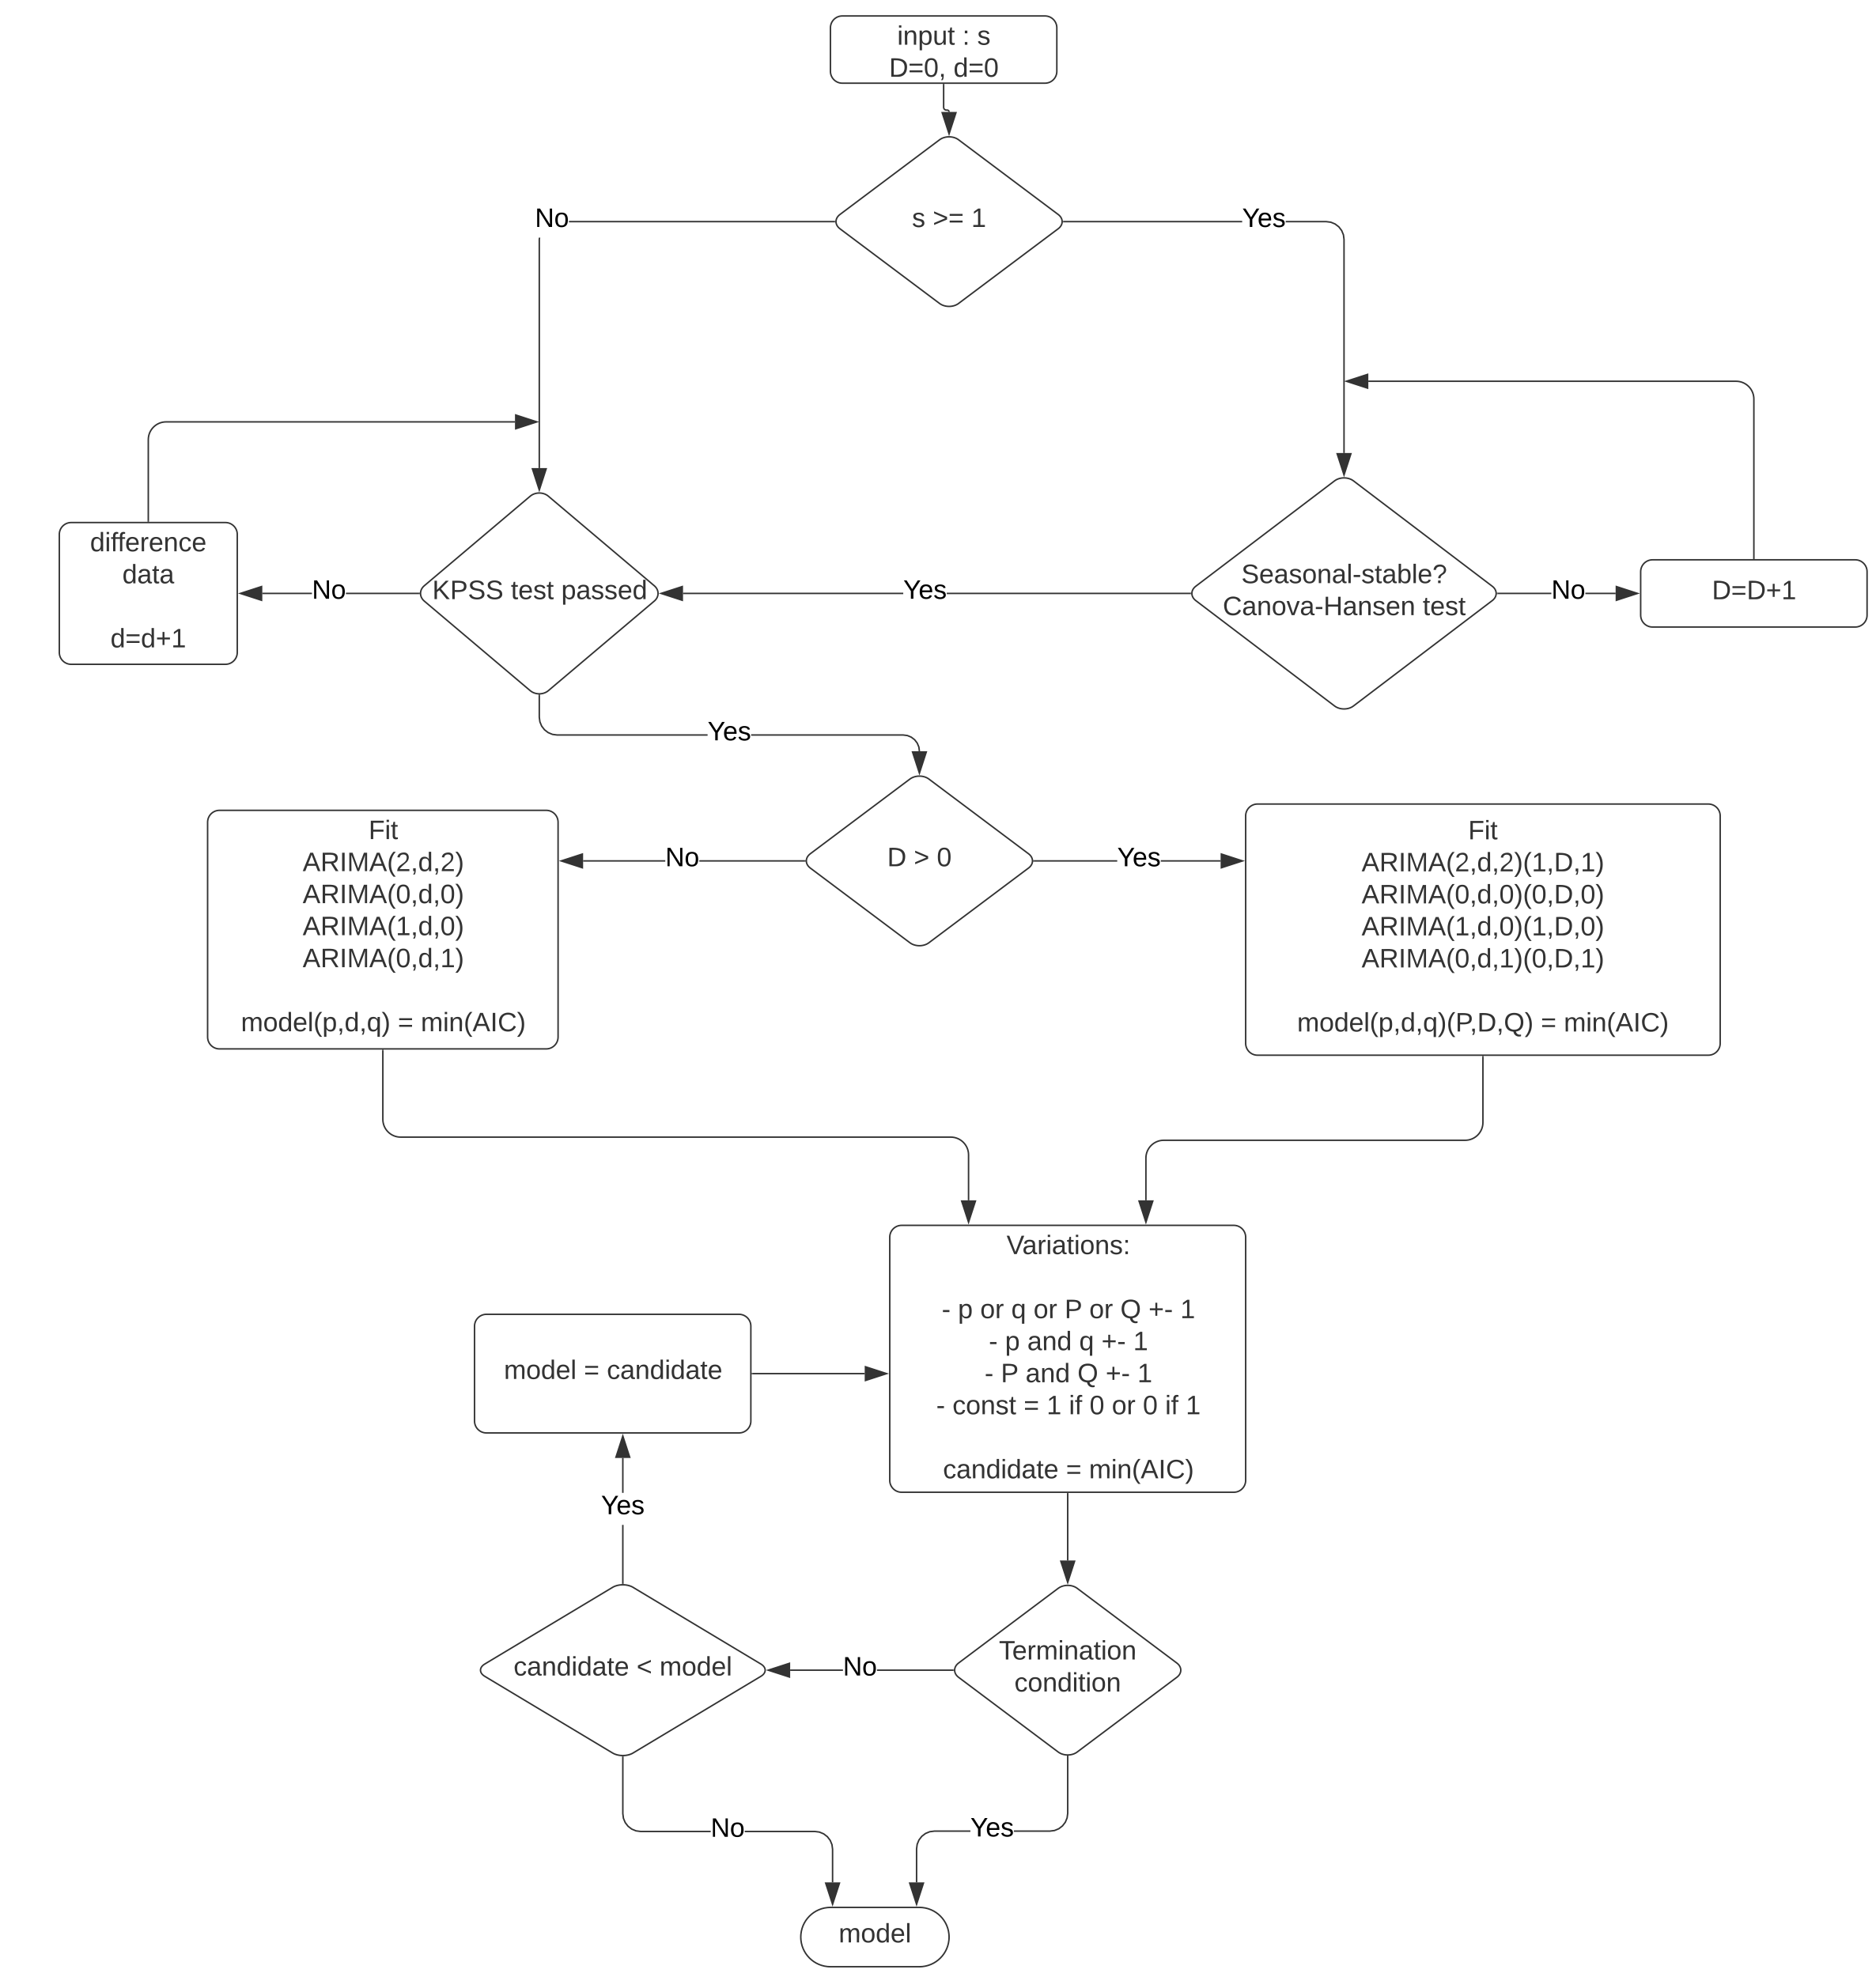
\includegraphics[width=\linewidth]{autoarima_algo}
	\caption{Hyndman-Khandakar algorithm for Auto-ARIMA estimation}
	\label{alg:autoarima}
\end{figure}
 
% \begin{figure}[H]
% 	\noindent\fbox{
% 		{\small\parbox{\textwidth}
% 			{
% 				\subsubsection*{Step 1: Find $D$ and $d$}
% 				
% 				For non-seasonal data run KPSS unit-root tests \cite{kpss}. If the results are significant difference the data and repeat $d$ times until the test results are insignificant. 
% 				
% 				For seasonal data it is considered ARIMA$(p,d,q)(P,D,Q)_s$ models where $s$ is the seasonal frequency and $D=0$ or $D=1$ depending on a extended Canova-Hansen test \cite{canovahansen} (for $s$ > 13 the library estimates critical values $C_s = 0.269s^{0.928}$). 
% 				
% 				After the seasonal pattern has passed its stability test and $D$ has been selected, $d$ is chosen by successive KPSS tests for seasonal differenced data if $D=1$, or the original data if $D=0$
% 				
% 				\subsubsection*{Step 2: Initial model}
% 				
% 				Fit the following models
% 				
% 				\begin{itemize}
% 					\item ARIMA$(2,d,2)$ if $s=1$ or ARIMA$(2,d,2)(1,D,1)$ if $s \geq 1$
% 					\item ARIMA$(0,d,0)$ if $s=1$ or ARIMA$(0,d,0)(0,D,0)$ if $s \geq 1$
% 					\item ARIMA$(1,d,0)$ if $s=1$ or ARIMA$(1,d,0)(1,D,0)$ if $s \geq 1$
% 					\item ARIMA$(0,d,1)$ if $s=1$ or ARIMA$(0,d,1)(0,D,1)$ if $s \geq 1$
% 				\end{itemize}
% 				
% 				From these ones it is selected the one with lowest AIC score as initial model, it will be called \emph{current} model and denoted as ARIMA$(p,d,q)$ if $s=1$ or ARIMA$(p,d,q)(P,D,Q)_s$ if $s \geq 1$
% 				
% 				\subsubsection*{Step 3: Explore variations}
% 				
% 				13 variations of current model are explored. They are summarised as: 
% 				
% 				\begin{itemize}
% 					\item One of $p, q, P$ and $Q$ is allowed to vary by $\pm1$ from the current model
% 					\item $p$ and $q$ vary both $\pm1$ from the current model
% 					\item $P$ and $Q$ both vary by $\pm1$ from the current model
% 					\item $c$ is included if the current model has $c=0$ or excluded if the current model has $c\neq0$.
% 				\end{itemize}
% 				
% 				Once it is found a model with better AIC score than the current model, then this one is updated. The algorithm stops when no better AIC than the current is found. 
% 				
% 				
% 				\emph{Note: The model updating is also subjected to stability constraints that can be found in the original publication for further details.}
% 				
% 			}
% 	}}
% 	\caption{Hyndman-Khandakar algorithm for Auto-ARIMA estimation}
% 	\label{alg:autoarima}
% \end{figure}


\section{Database construction pipeline}


A pipeline has been implemented to build a unified and non-corrupted database from the sparse-raw files so that the forecasting section could learn from reliable data. Figure \ref{fig:db_construction_algorithm} shows how the implemented blocks interact with each other to accomplish this task.

\begin{figure}[H]
	\centering
	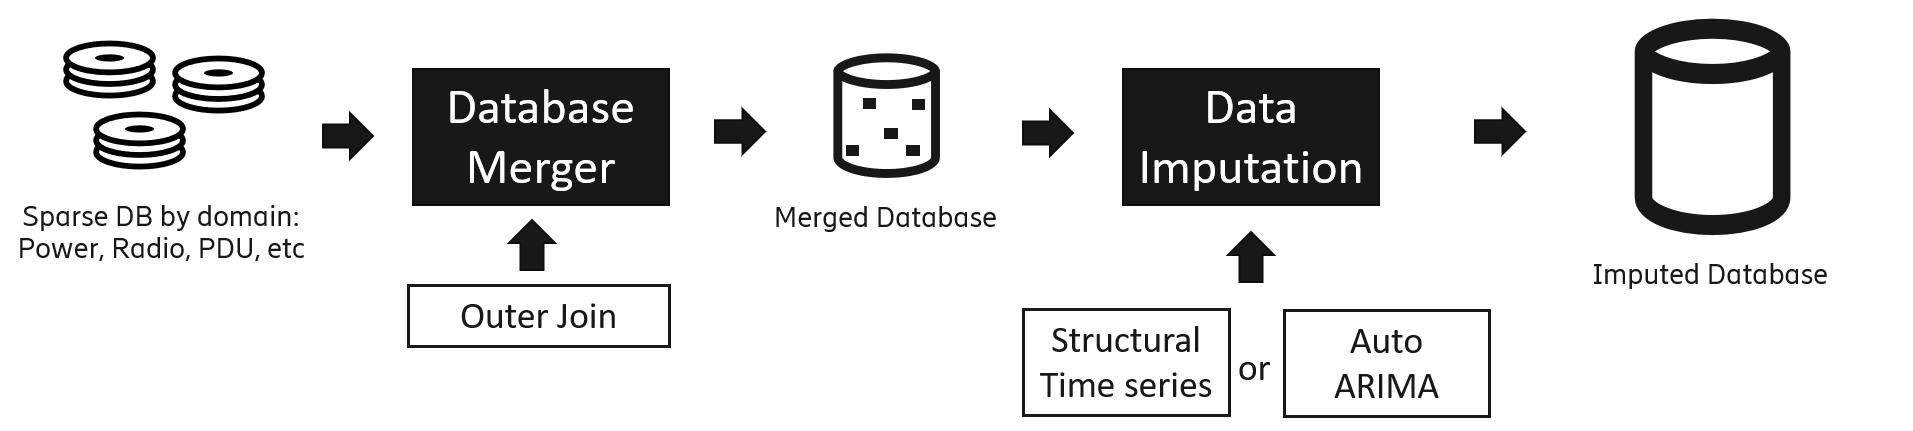
\includegraphics[width=0.8\linewidth]{db_construction_algorithm_final}
	\caption{Database construction algorithm}
	\label{fig:db_construction_algorithm}
\end{figure}







\section{Prophet fitting}

Prophet's Stan core \cite{carpenter2017stan} can be found in their GitHub repository\footnote{https://github.com/facebook/prophet} for further detailed research. The API exposes several more parameters to tune the models beyond the ones explained in Chapter \ref{cha:theory}. Some of them refer to the amount of \ac{mcmc} samples used to fit the trend, the limit of trend changepoints, the confidence interval size or some regularization variables used in the Stan model, among others.

%\begin{figure}[H]
%\begin{lstlisting}
%// Priors
%k ~ normal(0, 5);
%m ~ normal(0, 5);
%epsilon ~ normal(0, 0.5);
%delta ~ double_exponential(0, tau);
%beta ~ normal(0, sigma);
%
%// Logistic likelihood
%y ~ normal(C ./ (1 + exp(-(k + A * delta) .* (t - (m + A * gamma)))) + X * beta, epsilon);
%
%// Linear likelihood
%y ~ normal((k + A * delta) .* t + (m + A * gamma) + X * beta, sigma);
%\end{lstlisting}
%\caption{Prophet Stan model.}
%\label{alg:stan}
%\end{figure}

Another handy feature that allows using \acp{gam} is the ability to plot each component on its own, which allows the analyst to spot abnormalities when debugging a model. These plots will be shown and explained in Chapter \ref{cha:results}.



